\documentclass[10pt, oneside]{article}
\usepackage{amsmath, amsthm, amssymb, calrsfs, wasysym, verbatim, bbm, color, graphics, geometry}
\usepackage{pgfplots}
\pgfplotsset{compat=1.18}

\geometry{tmargin=.75in, bmargin=.75in, lmargin=.75in, rmargin = .75in}

\newcommand{\R}{\mathbb{R}}
\newcommand{\C}{\mathbb{C}}
\newcommand{\Z}{\mathbb{Z}}
\newcommand{\N}{\mathbb{N}}
\newcommand{\Q}{\mathbb{Q}}
\newcommand{\Cdot}{\boldsymbol{\cdot}}

\newtheorem{thm}{Theorem}
\newtheorem{defn}{Definition}
\newtheorem{conv}{Convention}
\newtheorem{rem}{Remark}
\newtheorem{lem}{Lemma}
\newtheorem{cor}{Corollary}


\title{ESMA 6605: Lecture Notes 1}
\author{Alejandro M. Ouslan}
\date{Lunes, 19 de Agosto de 2024}

\begin{document}

\maketitle
\tableofcontents

\vspace{.25in}

\section{Introduction a Estadisticas Matematicas}

\subsection{Que envuelve el analisis estadistico?}

\begin{itemize}
	\item Definir la pregunta de interes e identifica la poblacion
	\item Hacer el muestreo
	\item Recolectar el conjunto de datos en la muestra
	\item Organiar Resumir el conjunto de datos (\textbf{Estadisticca Descriptiva}: Medidas, descriptivas, tablas, graficas)
	\item Extrraer conclusiones sobre la poblacion a partir del conjunto de datos (\textbf{Estadistica Inferencial: Intervalos de Confianzo, Pruebas de Hipotesis}) asignado una medida de la fiabilidad de los resultados (usando \textbf{Prbabilidad})

\end{itemize}

\section{Muestreo}

\subsection{Muestreo Definisiones}
\begin{itemize}
	\item Queremos hacer inferencias sobre una poblacion
	\item Las muestras por convenienzas o muestras aliatorias puerden llevar a concluciones segadas (polarizadas)
	\item algunas observaciones pueden ocurrir mas frecuente que otras y vise versa.
	      \begin{defn}
		      Una muestrad de tamano $n$ es s
		      ionada al azar de modo que todas las muestras de tamano $n$ tiene la misma probabilidad de ser seleccionadas.
	      \end{defn}
\end{itemize}

\subsection{sd}
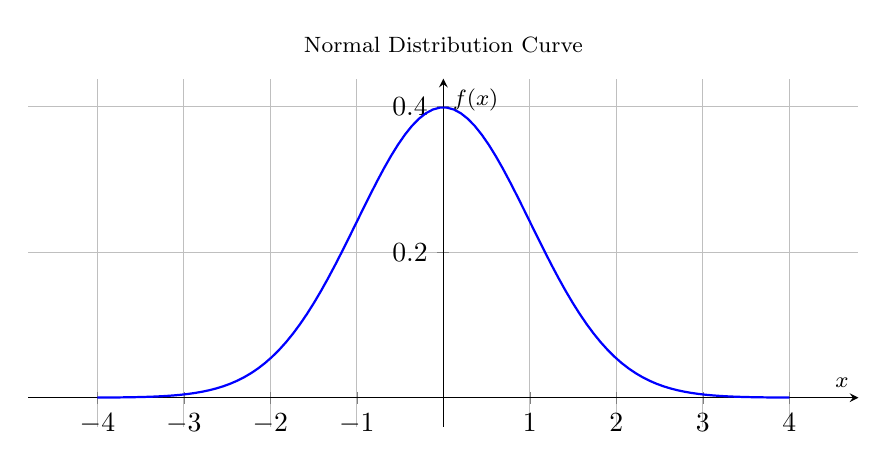
\begin{tikzpicture}
	\begin{axis}[
			axis lines = middle,
			xlabel = $x$,
			ylabel = $f(x)$,
			title = Normal Distribution Curve,
			domain = -4:4,
			samples = 100,
			width = \textwidth,
			height = 6cm,
			xlabel style = {font=\footnotesize},
			ylabel style = {font=\footnotesize},
			title style = {font=\footnotesize},
			grid = major,
			restrict y to domain = 0:1,
			enlargelimits
		]
		\addplot[
			thick,
			blue
		]
		{exp(-x^2/2) / sqrt(2*pi)};
	\end{axis}
\end{tikzpicture}
\end{document}
